\graphicspath{{images/}}

\section{Ход работы}

Я выбрал набор данных Predicting Heart Failure \cite{kaggle} для выполнения лабораторной работы. В описании датасета предлагается
предсказать, будет ли в ближайшее время у человека сердечный приступ или нет.
Признаки в наборе данных:

\begin{enumerate}
    \item
    age --- возраст человека, который находится пол наблюдением
    \item
    anaemia --- показатель есть ли у наблюдаемого пациента анемия.
    \item
    high blood pressure --- показатель, повышенное ли у человека давление.
    \item
    creatinine phosphokinase --- уровень CPK в крови человека, числовой признак.
    \item
    diabetes --- есть ли у пациента диабет.
    \item
    ejection fraction --- процент крови, покидающее сердце после каждого удара, выражается в процентах, числовой признак.
    \item
    platelets --- количество тромбоцитов в крови, числовой признак.
    \item
    sex --- пол пациента.
    \item
    serum creatinine --- количество креатинина в сыворотке крови человека.
    \item
    serum sodium --- количество натрия в сыворотке крови человека.
    \item
    smoking --- курящий человек или нет.
    \item
    time --- количество дней под наблюдением.
    \item
    DEATH\_EVENT --- целевая переменная, указывает, проищошёл ли сердечный приступ в итоге или нет.
\end{enumerate}

Перед выявлением зависимостей между признаками следует проверяю целостность набора данных:
\begin{alltt}
<class 'pandas.core.frame.DataFrame'>
RangeIndex: 299 entries, 0 to 298
Data columns (total 13 columns):
 #   Column                    Non-Null Count  Dtype  
---  ------                    --------------  -----  
 0   age                       299 non-null    float64
 1   anaemia                   299 non-null    int64  
 2   creatinine_phosphokinase  299 non-null    float64
 3   diabetes                  299 non-null    int64  
 4   ejection_fraction         299 non-null    float64
 5   high_blood_pressure       299 non-null    int64  
 6   platelets                 299 non-null    float64
 7   serum_creatinine          299 non-null    float64
 8   serum_sodium              299 non-null    float64
 9   sex                       299 non-null    int64  
 10  smoking                   299 non-null    int64  
 11  time                      299 non-null    float64
 12  DEATH_EVENT               299 non-null    int64  
dtypes: float64(7), int64(6)
memory usage: 30.5 KB
\end{alltt}

В наборе нет неполных данных, а все признаки - числовые.
\pagebreak

Построю графики для каждой пары признаков. Синим отмечен успех, оранжевым - неуспех:
\begin{center}
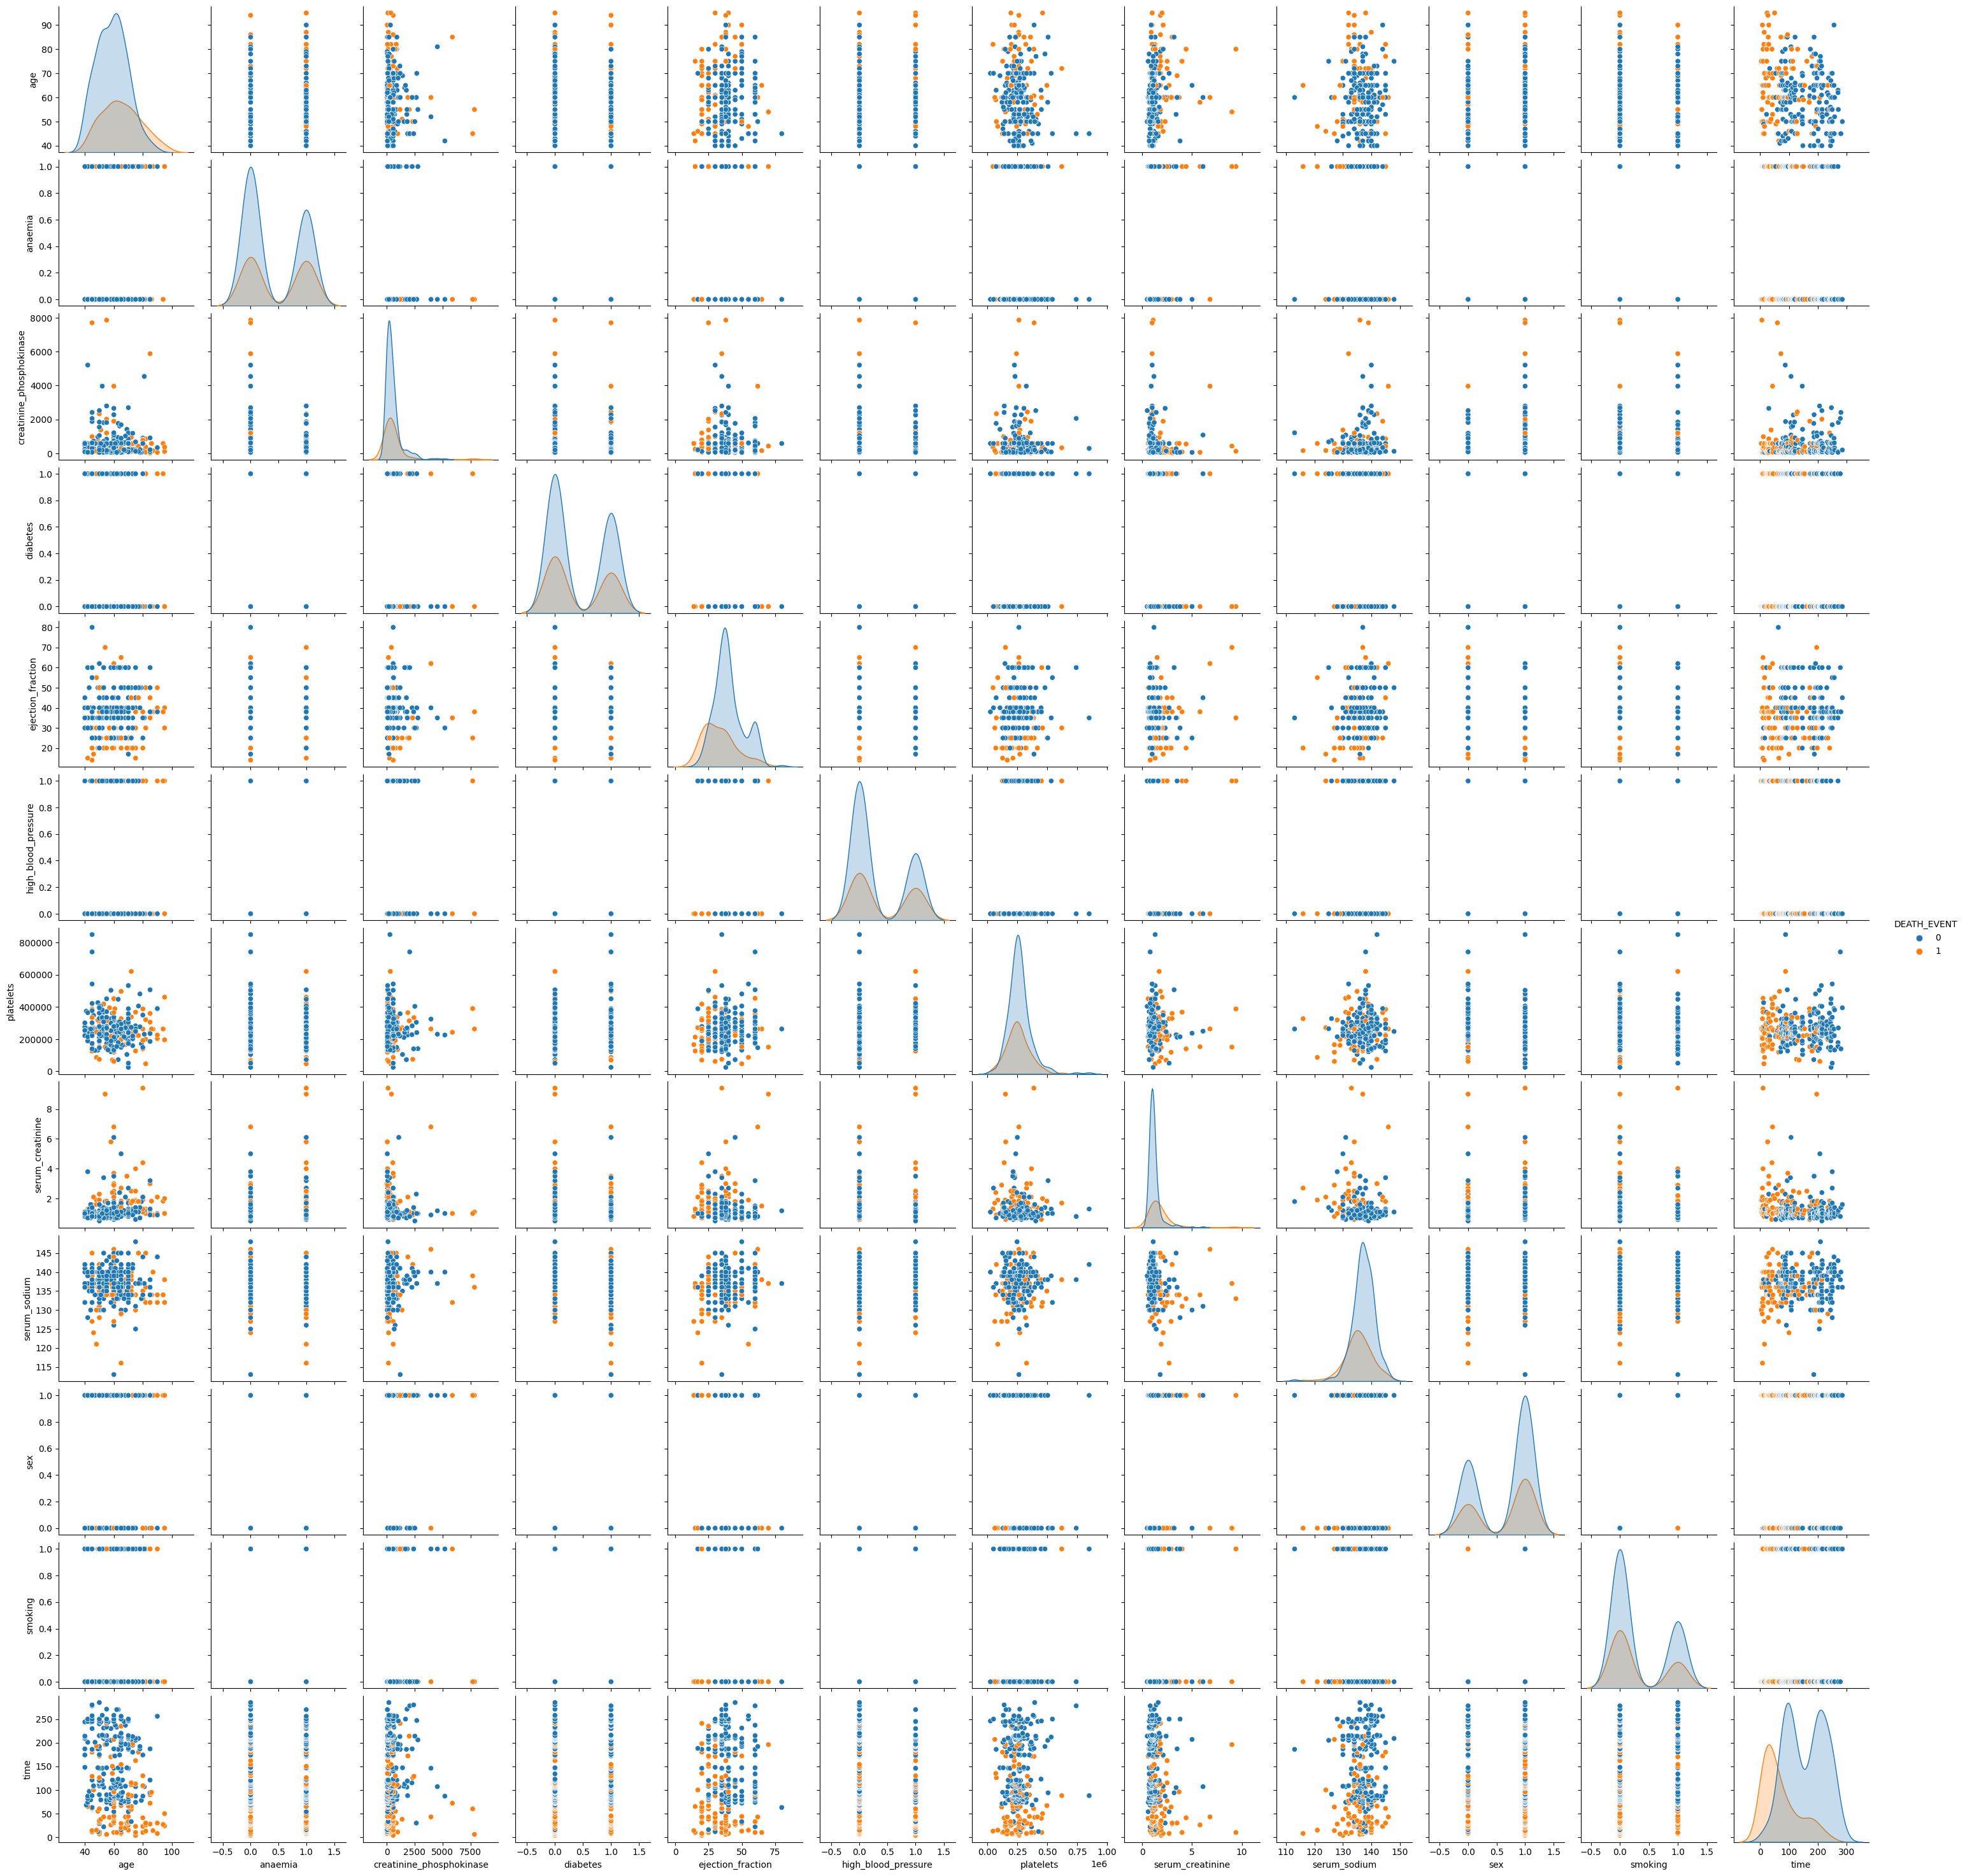
\includegraphics[scale=0.20]{pair}
\end{center}\pagebreak

Построю корреляционную матрицу для признаков:
\begin{center}
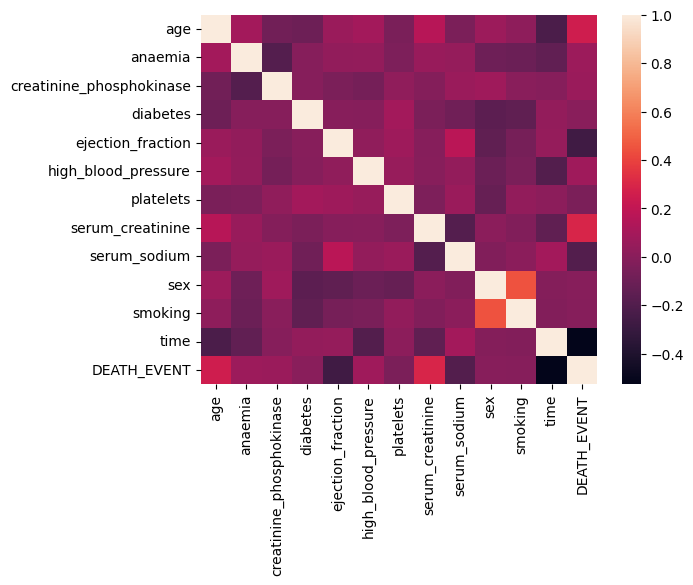
\includegraphics[scale=0.65]{corr}
\end{center}
Так же построю гистограммы для числовых признаков:
\begin{center}
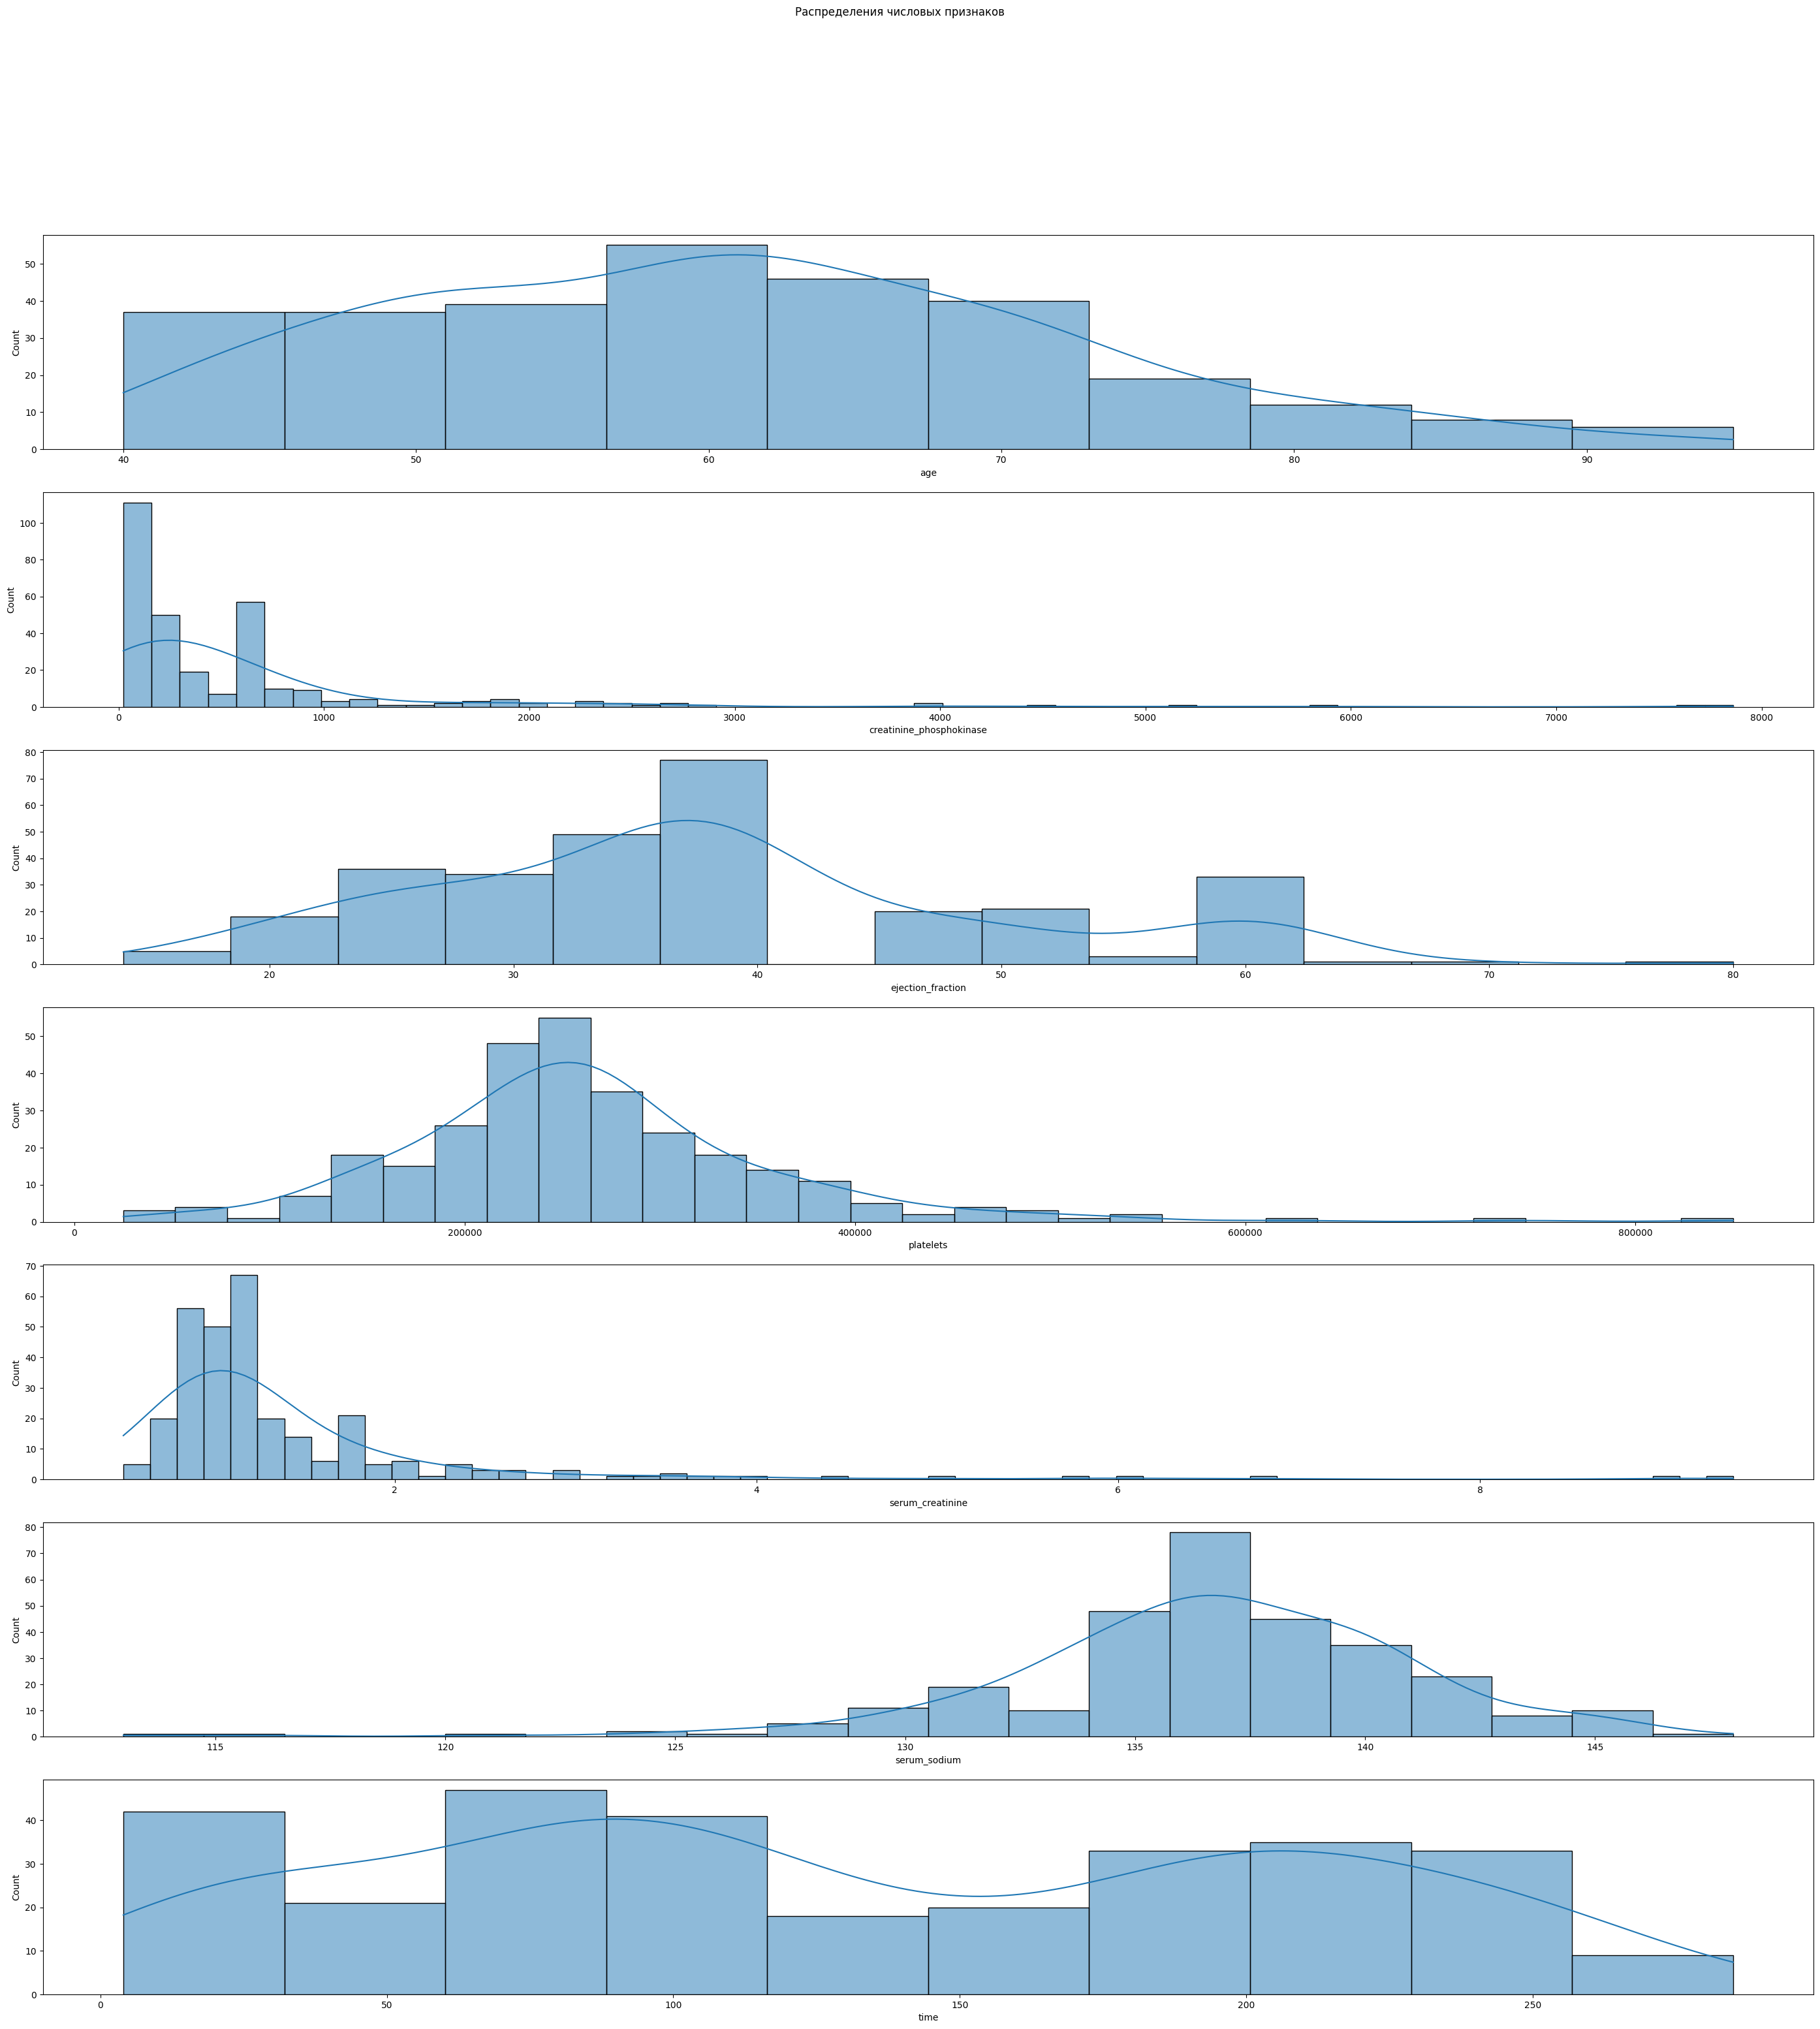
\includegraphics[scale=0.15]{bar}
\end{center}
Выбросов не было обнаружено, так как датасет довольно маленький.
\pagebreak

Соотношение классов объектов:
\begin{center}
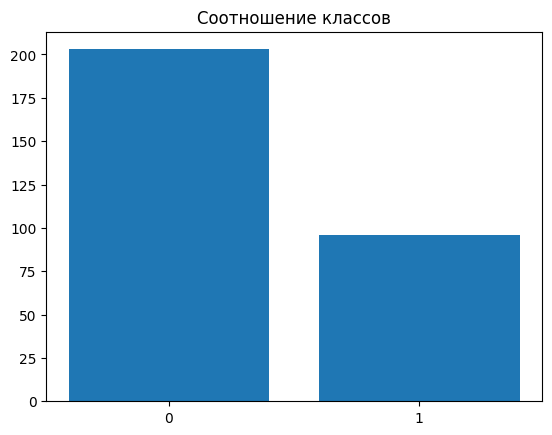
\includegraphics[scale=0.65]{classes}
\end{center}
Количество объектов разных классов заметно различается, сделаем RandomOversampling при помощи imbalanced-learn, это позволит не прибегать
к неточным синтетическим данным, при этом наши данные будут лучше подходить для обработки алгоритмами классического МЛ. 
Данные готовы к обучению.

\pagebreak
